\newpage
\part{Web Processing Service}
\newpage
\section{Web Processing Service}

\subsection{History}
The first mention of the Web Processing Service was in October 2004. Back then it
was named Geoprocessing Service \cite{OGC_news}. The specification was first 
implemented as a prototype in 2004 by Agriculture and Agri-Food Canada (AAFC).
In its further development during a Geoprocessing Services Interoperability Experiment \cite{WPS_experiment} 
the name was changed to "Web Processing Service" to avoid the acronym GPS, since 
this would have caused confusion with the conventional use of this acronym for 
Global Positioning System \cite{WPS_standart_1.0}. The first version of WPS was released in
September 2005 \cite{WPS_first}. The experiment demonstrated that various clients
could easily access and bind to services which were set up according to the WPS Implementation
specification.

Currently two major versions of WPS Standard exist. The WPS version 1.0.0 is currently most used.
If not explicitly said this thesis is dedicated to the version 1.0.0. The WPS version 2.0.0 was
released in 2015 \cite{WPS_second}.

\subsection{Open Geospatial Consortium}
The OGC \textit{Open Geospatial Consortium} is an international non-profit organization committed to making quality 
open standards for the global geospatial community. These standards are made through a consensus process and are freely available for anyone to use. The OGC members come from government, commercial organizations, NGOs, academic and research organizations.\cite{OGC}

A predecessor organization, OGF, the Open GRASS Foundation, started in 1992. From 1994 the organization 
used the name \textit{Open GIS Consortium}, in 2004 the Board changed the name to \textit{Open Geospatial Consortium}.\cite{OGC_history}

Some of the widely-use OGC standards are:
\begin{itemize}
\item WCS, WMS, WFS, WMTS or WPS - standards for web services
\item GML, KML - standards for XML-based languages
\end{itemize}


\bigskip
\subsection{Web Processing Service}
The OGC Web Processing Service (WPS) Interface Standard defines a standardized interface
that facilitates the publishing of geospatial processes. Also provides rules how to standardize
requests and responses for geospatial processing services. 

\textit{Process} means any operation on spatial
%% ML: as -> like ?
%% AL: opraveno
data from simple ones like maps overlay or buffering to highly complex as complicated global models. Any kind of GIS 
functionality can be offered to clients across a network with correctly configured WPS. 

\textit{Publishing} means
creating human-readable metadata that allow users to discover and use service as well as making 
available machine-readable binding information.

\textit{Data} can be both vector or raster data and can be delivered across the network or be available
at the server.

The interface does not specify any specific processes that can be implemented by a WPS nor any specific
data inputs or outputs. Instead it specifies generic mechanisms to describe any geospatial process and
data required and produced by the process. The interface does not only provide mechanisms for calculation
but also mechanisms that identify required data, initiate the calculation and manage output data so clients
can access it. 

\bigskip
Web Processing Service as one of the OGC web services specifies three types of requests which can be requested
by a client and performed by a WPS server. The implementation of these three requests is mandatory by all servers:

\textbf{\textit{GetCapabilities}} - The request returns to the client a Capabilities document that describes the abilities
of the specific server implementation. It also returns the name and abstract of each of the processes that can
be run on a WPS instance.

\textbf{\textit{DescribeProcess}} - The request returns details about the processes offered by a WPS instance. 
It describes required inputs and produced outputs and their allowable formats.

\textbf{\textit{Execute}} - The request allows the client to run a specified process with provided parameters and returns
produced outputs.

\newpage
These operations are very similar to other OGC Web Services such as WMS, WFS, and WCS. Common interface aspects
are defined in the OGC Web Services Common Implementation Specification \cite{OGC_common}. As seen in 
the class diagram at Fig. \ref{fig:WPS_class_diagram} the~WPS interface class inherits the GetCapabilities operation 
from OGCWebService interface class. The operations Execute and DescribeProcess are specific for the WPS. The WPS
%% ML: vysvetlit v poznamce pod carou co je get a post?
%% AL: vysvetleno.
operations are based on HTTP GET\footnote{\textit{HTTP GET} requests data from a specified resource. Data are sent in the URL of a GET request.} and 
POST\footnote{\textit{HTTP POST} submits data to be processed to a specified resource. Data are sent inside the HTTP message body of
POST request} requests.

\begin{figure}[h!]
\centering
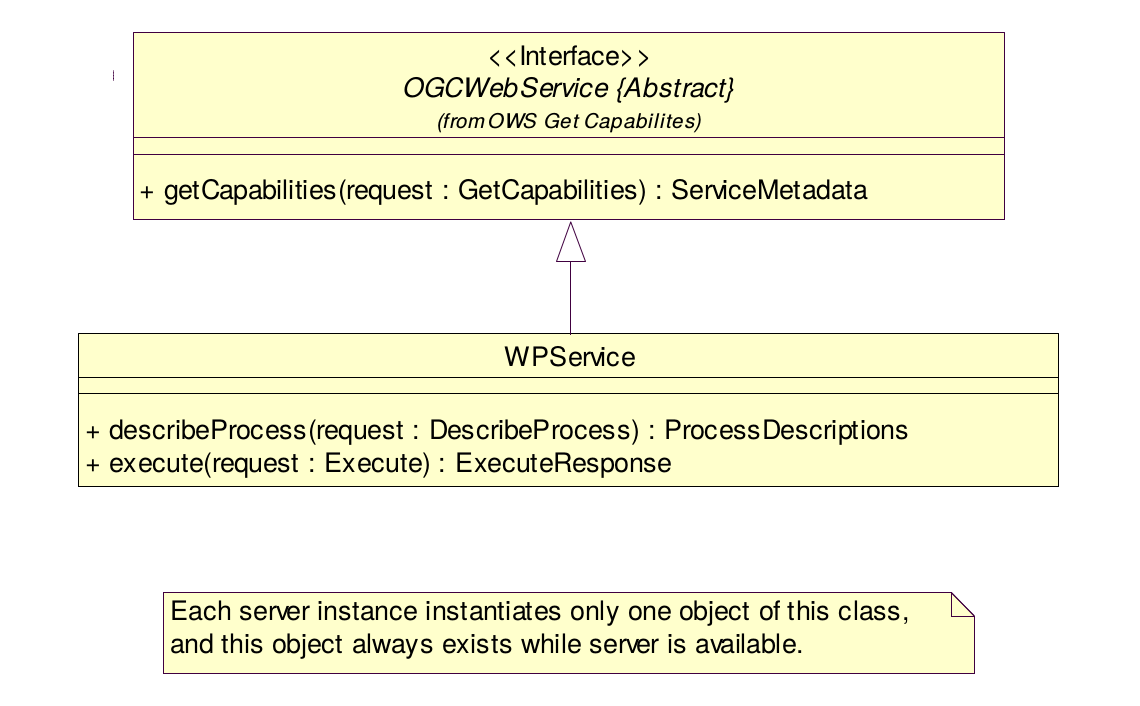
\includegraphics[width=0.78\textwidth]{img/WPS_class_diagram.png}
\caption{WPS interface UML description, source: \cite{WPS_standart_1.0}}
\label{fig:WPS_class_diagram}
\end{figure}

%% ML: mas nekde vystetleno co je KVP a XML encoding?
%% AL: vysvetleno.
The GetCapabilities and DescribeProcess shall use HTTP GET with KVP encoding and Execute operation shall use HTTP
POST with XML encoding. Summarized in Tab. \ref{tab:WPS_encoding}.
\begin{table}[h!]
\catcode`\-=12
\centering
\begin{tabular}{|c|c|c|}
\hline
%% ML: proc je hlavicka mensim pismem?
%% AL: mne se hlavicka vykresluje stejne velkym pismem.
\multirow{2}{*}{Operation} & \multicolumn{2}{c|}{Request encoding} \\ \cline{2-3} 
                           & Mandatory          & Optional         \\ \hhline{|=|=|=|}
GetCapabilities            & KVP                & XML              \\ \hline
DescribeProcess            & KVP                & XML              \\ \hline
Execute                    & XML                & KVP              \\ \hline
\end{tabular}
\caption{Operations request encoding}
\label{tab:WPS_encoding}
\end{table}


\paragraph{KVP encoding} are key-value pairs usually sent via HTTP GET request method encoded directly in the URL. The 
keys and values are separated with = sign and each pair is separated with \& sign  or with ? sign at the beginning of 
the request. Example could be the get capabilities request:

\begin{lstlisting}[basicstyle=\small,caption={GetCapabilities with KVP encoding.}]
http://server.domain/wps?service=WPS&request=GetCapabilities&version=1.0.0
\end{lstlisting}

In this example, there are 3 pairs of input parameter: service, request and version with values WPS, GetCapabilities and 
1.0.0 respectively.\cite{PyWPS_docs}

\paragraph{XML payload} is XML data sent via HTTP POST request method. The XML document can be more rich, having more 
parameters, better to be parsed in complex structures. The Client can also encode entire datasets to the request, 
including raster (encoded using base64) or vector data (usually as GML file).\cite{PyWPS_docs}

\begin{lstlisting}[basicstyle=\small,caption={GetCapabilities XML payload example}]
<?xml version="1.0" encoding="UTF-8"?>
<wps:GetCapabilities language="cz" service="WPS" xmlns:ows="http://www.opengis.net/ows/1.1" xmlns:wps="http://www.opengis.net/wps/1.0.0" xmlns:xsi="http://www.w3.org/2001/XMLSchema-instance" xsi:schemaLocation="http://www.opengis.net/wps/1.0.0 http://schemas.opengis.net/wps/1.0.0/wpsGetCapabilities_request.xsd">
  <wps:AcceptVersions>
    <ows:Version>1.0.0</ows:Version>
  </wps:AcceptVersions>
</wps:GetCapabilities>
\end{lstlisting}

\subsubsection{GetCapabilities}
The GetCapabilities operation is mandatory. The operation allows a client to retrieve capabilities document (metadata)
from a server. The response XML document contains service metadata about the server and all implemented processes description.

\paragraph{GetCapabilities request}

\begin{table}[h!]
\catcode`\-=12
\centering
\begin{tabular}{|c|c|c|}
\hline
\thead{Name}               & \thead{Optionality and use} & \thead{Definition and format}    		\\ \hhline{|=|=|=|}
service=WPS                & Mandatory           & Service type identifier text 	\\ \hline
request=GetCapabilities    & Mandatory           & Operation name text              \\ \hline
AcceptVersion=1.0.0        & Optional            & Specification version            \\ \hline
Sections=All               & Optional            & \makecell{Comma-separated \\unordered list of sections} \\ \hline
updateSequence=XXX         & Optional            & \makecell{Service metadata \\document version}            \\ \hline
AcceptFormats=text/xml     & Optional            & \makecell{Comma-separated prioritized \\sequence of response formats} \\ \hline
\end{tabular}
\caption{GetCapabilities operation request URL parameters, source: \cite{OGC_common}}
\label{tab:WPS_GetCapabilities}
\end{table}

\begin{itemize}
\item\textit{service} - A mandatory parameter, WPS is only possible value.
\item\textit{request} - A mandatory parameter, GetCapabilities is only possible value.
\item\textit{version} - An optional parameter, version number. Three non-negative integers separated by a decimal point. Servers and
their clients should support at least one defined version.
\item\textit{sections} - An optional parameter that contains a list of section names. Possible values are: \textit{ServiceIdentification,
ServiceProvider, OperationsMetadata, Contents, All}.
\item\textit{updateSequence} - An optional parameter for maintaining the consistency of a~client cache of the contents of a service
metadata document. The parameter value can be an integer, a timestamp, or any other number or string.
\item\textit{format} - An optional parameter that defines response format.
\end{itemize}

A client can request the GetCapabilities operation with parameters from the Tab. \ref{tab:WPS_GetCapabilities}. A corresponding
request URL looks like:

\noindent
\url{http://localhost:5000/wps?service=WPS&request=GetCapabilities&AcceptVe}\\
\url{rsion=1.0.0&Section=ServiceIdentification,OperationsMetadata&updateSeq}\\
\url{uence=XXX&AcceptFormats=text/xml}

\paragraph{GetCapabilities response}
\label{para:GetCapa_response}
%% ML: co znamena Normal?
%% AL: jakoze neskonci s exception. Ale mozna je ten nadpis matouc, mazu
When GetCapabilities operation is requested a client retrieve service metadata document that contains sections specified in
\textit{sections} parameter. If the parameter value is \textit{All} or not specified than all sections are retrieved.

\begin{itemize}
\item\textit{ServiceIdentification} - Server metadata.
\item\textit{ServiceProvider} - Server operating organization metadata.
\item\textit{OperationsMetadata} - Metadata about operations implemented by the WPS server, including URLs to request them.
\item\textit{ProcessOfferings} - List of processes with name and brief description implemented by the WPS server.
\end{itemize}

\bigskip
In addition to sections each GetCapabilities response should contain:
\begin{itemize}
\item\textit{version} - Specification version for GetCapabilities operation.
\item\textit{updateSequence} - Server metadata document version, value is increased whenever any change is made in complete service metadata document.
\end{itemize}

\subparagraph{GetCapabilities exceptions}
In case that WPS server encounters an error a~client retrieves an exception report message with one of the exception code:

\begin{itemize}
\item\textit{MissingParameterValue} - GetCapabilities request does not contain a required parameter value.
\item\textit{InvalidParameterValue} - GetCapabilities request contains an invalid parameter value.
\item\textit{VersionNegotiation} - Any version from AcceptVersions parameter list does not match any version supported by the WPS server.
\item\textit{InvalidUpdateSequence} - Value of updateSequence parameter is greater than current value of service metadata updateSequence number.
\item\textit{NoApplicableCode} - Other exceptions.
\end{itemize}

\subsubsection{DescribeProcess}
The DescribeProcess operation is mandatory. The operation allows clients to retrieve a detailed description of one or more
processes implemented by a WPS server. The detailed information describes both required inputs and produced outputs and allowed
formats.

\begin{table}[h!]
\catcode`\-=12
\centering
\begin{tabular}{|c|c|c|}
\hline
\thead{Name}               & \thead{Optionality} & \thead{Definition and format}    		\\ \hhline{|=|=|=|}
service=WPS                & Mandatory           & Service type identifier text 	\\ \hline
request=DescribeProcess    & Mandatory           & Operation name text              \\ \hline
version=1.0.0              & Mandatory           & WPS specification version            \\ \hline
Identifier=buffer          & Optional            & \makecell{List of one or more process\\ identifiers, separated by commas} \\ \hline
\end{tabular}
\caption{DescribeProcess operation request URL parameters, source: \cite{OGC_common}}
\label{tab:WPS_DescribeProcess}
\end{table}

\paragraph{DescribeProcess request}
\begin{itemize}
\item\textit{service} - Mandatory parameter, WPS is only possible value.
\item\textit{request} - Mandatory parameter, DescribeProcess is only possible value.
\item\textit{version} - Mandatory parameter, version number. Three non-negative integers separated by decimal point. Servers and
their clients should support at least one defined version.
\item\textit{Identifier} - Optional parameter, list of process names separated by comma. Another possible value is \textit{all}.
\end{itemize}

The DescribeProcess operation can be requested with parameters from Tab. \ref{tab:WPS_DescribeProcess}. A corresponding
request URL looks like: \url{http://localhost:5000/wps?request=DescribeProcess&service=WPS&identifier=all&version=1.0.0}

\paragraph{DescribeProcess response}
\label{para:DesribeProc_response}

%% ML: Normal? viz poznamka vyse
%% AL: Smazano
A response to DescribeProcess request contains one or more process descriptions for requested process identifiers.
%% ML: co to je za strukturu, zde poprve pouzivas kurzivu, z toho mam pocit, ze jde o neco podstatneho ;-)
%% ML: nikde jinde o strukture nemluvis, to je matouci
%% AL: prepsal jsem odstavec, snad je to srozumitelnejsi
Each
process description contains detailed information about process in ProcessDescription XML element (see Tab. 
\ref{tab:WPS_ProcessDescription})
including process inputs and outputs description. The number of inputs or outputs is not limited.

\bigskip
\begin{table}[h!]
\catcode`\-=12
\centering
\begin{tabular}{|c|c|c|}
\hline
\thead{Name}               & \thead{Optionality} & \thead{Definition and format}    		\\ \hhline{|=|=|=|}
Identifier      	       & Mandatory           & Process identifier             \\ \hline
Title 			           & Mandatory           & Process title 				  \\ \hline
Abstract		           & Optional            & Brief description              \\ \hline
Metadata		           & Optional            & \makecell{Reference to more metadata about this process} \\ \hline
Profile			           & Optional            & \makecell{Profile to which the WPS process complies} \\ \hline
processVersion	           & Mandatory           & Release version of process \\ \hline
WSDL    		           & Optional            & \makecell{Location of a WSDL document that \\describes this process} \\ \hline
DataInputs		           & Optional            & \makecell{List of the required and optional inputs} \\ \hline
ProcessOutputs	           & Mandatory           & \makecell{List of the required and optional outputs} \\ \hline
storeSupported	           & Optional            & \makecell{Complex data outputs can be \\stored by WPS server} \\ \hline
statusSupported	           & Optional            & \makecell{Execute response can be returned\\ quickly with status information} \\ \hline
\end{tabular}
\caption{Parts of ProcessDescription data structure, source: \cite{WPS_standart_1.0}}
\label{tab:WPS_ProcessDescription}
\end{table}

\noindent
Three data types of input or outputs exist:
\begin{itemize}
\item\textit{LiteralData} - any string. It is used for passing single parameters like numbers or text parameters. There can be set
\textit{allowedValues} restriction. It can be a~list of allowed values or input data type. Additional attributes such as \textit{units}
or \textit{encoding} can be set as well. 
\item\textit{ComplexData} - Complex data can be raster, vector or any file-based data, which are usually processed. ComplexData
%% ML: vysvetlit mimeType, poznamka pod carou?
%% AL: vysvetleno
are often result of the process. The input can be specified more using 
mimeType\footnote{\textit{mimeType} - is a standardized way to indicate the nature and format of a document. Browsers often use the MIME type (and not the file extension) to determine how it will process a document.}, XML schema or encoding.
\item\textit{BoundingBoxData} - BoundingBox data are specified in OGC OWS Common specification as two pairs of 
coordinates (for 2D and 3D space). They can either be encoded in WGS84 or EPSG code can be passed too. They are intended 
to be used as definition of the target region.
\end{itemize}

\subparagraph{DescribeProcess exceptions}
In case that WPS server encounters an error a~client retrieves an exception report message with one of the exception code:
\begin{itemize}
\item\textit{MissingParameterValue} - GetCapabilities request does not contain a required parameter value.
\item\textit{InvalidParameterValue} - GetCapabilities request contains an invalid parameter value.
\item\textit{NoApplicableCode} - Other exceptions.
\end{itemize}

\subsubsection{Execute}
The Execute operation is mandatory. The operation allows clients to run a specified process implemented by a server.
Inputs can be included directly in the request body or be referenced as a web-accessible resource. The outputs are 
returned in XML response document, either directly embedded within the response document or stored as a resource 
accessible by returned URL.

\bigskip
\begin{table}[h!]
\catcode`\-=12
\centering
\begin{tabular}{|c|c|c|}
\hline
\thead{Name}               & \thead{Optionality} & \thead{Definition and format}    		\\ \hhline{|=|=|=|}
service          	       & Mandatory           & Service type identifier text             \\ \hline
request			           & Mandatory           & Operation name text 				  \\ \hline
version			           & Mandatory           & WPS specification version              \\ \hline
Identifier   	           & Mandatory           & Process identifier \\ \hline
DataInputs		           & Optional            & \makecell{List of inputs provided \\ to this process execution} \\ \hline
ResponseForm	           & Optional            & Response type definition \\ \hline
language   		           & Optional            & Language identifier \\ \hline
\end{tabular}
\caption{Parts of Execute operation request, source: \cite{WPS_standart_1.0}}
\label{tab:WPS_ExecuteRequest}
\end{table}

%% ML: OK, tady uz zadne Normal neni... :-)
\paragraph{Execute request}
%% ML: Zkus odstavec prepsat, je to utrzkovite...
%% AL: trochu prehazena struktura a prepsany text
Execute request is usually sent via HTTP POST request. It triggers an execution of a specified process if no exceptions
raised (for instance ServerBusy). Execute request contains parameters from Tab. \ref{tab:WPS_ExecuteRequest}. Example of 
Execute XML response document sent within the POST request can be found at App. \ref{app:ExecuteRequest}. 


\paragraph{Execute response}
Usually the Execute operation response document is an XML document. The only exception is in case when a response form
of \textit{RawDataOutput} is requested, execution is successful and only one complex output is created, then directly
the produced complex output is returned. The result can be inserted directly inline the response document or be
referenced as web-accessible resource, it depends on ResponseForm request elements.

\begin{figure}[h!]
\centering
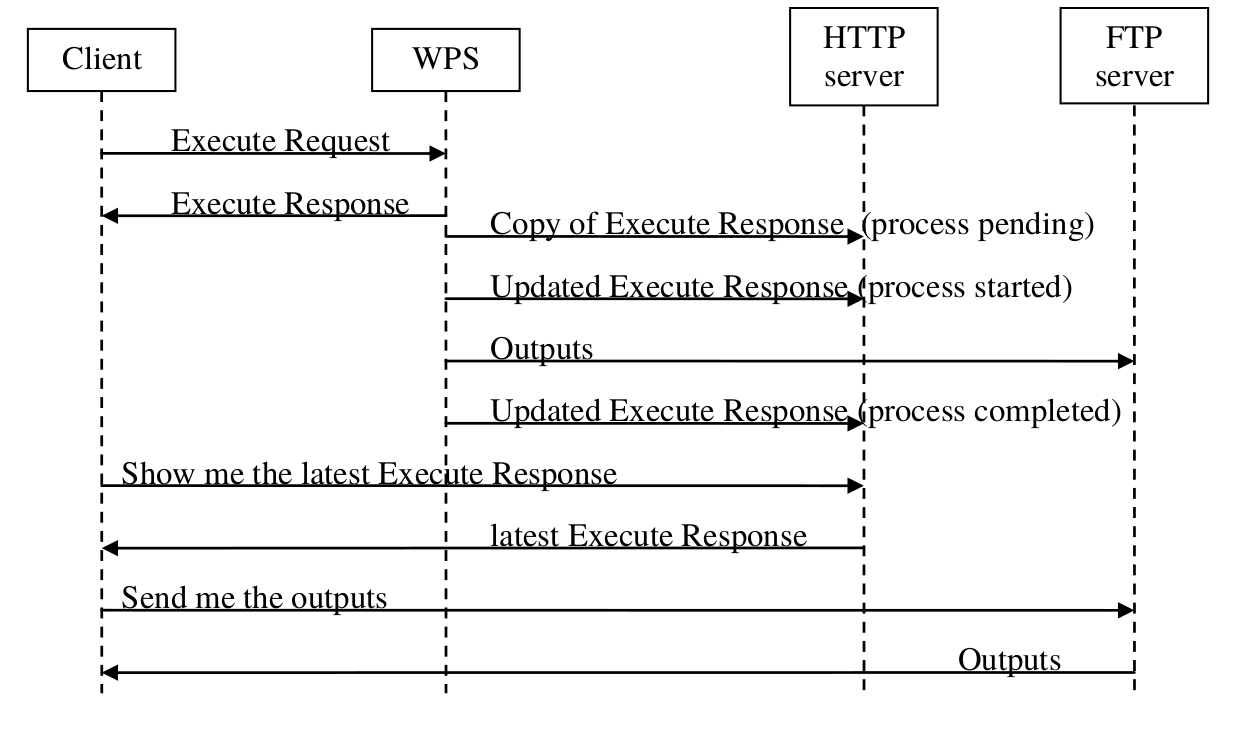
\includegraphics[width=0.8\textwidth]{img/WPS_sequence.png}
\caption{Sequence diagram: a client requests storage of results, source: \cite{WPS_standart_1.0}}
\label{fig:WPS_sequence}
\end{figure}

%% ML: right after hned ve dvou vetach po sobe...
%% AL: opraveno
In synchronous mode the response document is returned when the process execution is completed. However in asynchronous
mode it is possible to get
response document right after sending a request. In this case, returned response document contains a URL link from which 
the final response document can be retrieved after completed process execution. A~client can request execution status 
update to find out the amount of processing remaining if the execution is not completed. Shown in Fig. 
\ref{fig:WPS_sequence}.

%% ML: Podobna veta je na zacatku predesleho odstavce
%% AL: Prepsano.


\newpage
\begin{table}[h!]
\catcode`\-=12
\centering
\begin{tabular}{|c|c|c|}
\hline
\thead{Name}               & \thead{Optionality} & \thead{Definition and format}    		\\ \hhline{|=|=|=|}
service          	       & Mandatory           & Service type identifier text             \\ \hline
version			           & Mandatory           & WPS specification version              \\ \hline
language   		           & Mandatory           & Language identifier \\ \hline
statusLocation	           & Optional            & \makecell{Reference to location where current\\ExecuteResponse document is stored} \\ \hline
serviceInstance	           & Mandatory           & \makecell{Reference to location where current\\ExecuteResponse document is stored} \\ \hline
Process			           & Mandatory           & Process description \\ \hline
Status			           & Mandatory           & Execution status of the process \\ \hline
DataInputs		           & Optional            & \makecell{List of inputs provided \\ to this process execution} \\ \hline
OutputDefinitions          & Optional            & \makecell{List of definitions of outputs \\desired from executing this process} \\ \hline
ProcessOutputs             & Optional            & \makecell{List of values of outputs \\ from process execution} \\ \hline
\end{tabular}
\caption{Parts of ExecuteResponse data structure, source: \cite{WPS_standart_1.0}}
\label{tab:WPS_ExecuteResponse}
\end{table}

\newpage
\section{WPS implementations}
The OGC WPS is just an interface standard that provides rules for
%% ML: requests (mnozne cislo), response (jednotne) - je v tom nejaky zamer?
%% AL: opraveno
standardizing requests and responses. It also defines how clients can
request the execution of defined processes and how the outputs are
handled. There are several projects that implement this standard
across the platforms or programming languages.

\subsection{deegree}

%% ML: their zni v odstavci divne
%% AL: opraveno
\textit{deegree} is open-source community-driven project for spatial
data infrastructure written in Java. Besides from the other OGC Web
Services it implements also WPS standard 1.0.0. The implementation offers
sending request with KVP, XML or SOAP encoding,
asynchronous/synchronous execution and API for implementing processes
in Java. On their website there is a WPS demo
\footnote{\url{http://demo.deegree.org/wps-workspace/}} where all
operations \textit{GetCapabilities}, \textit{DescribeProcess} and
\textit{Execute} with various processes can be tested.

\bigskip
\begin{figure}[h!]
\centering

\includegraphics[width=0.2\textwidth]{img/deegree.png}
\caption{deegree project logo}
\label{fig:deegree}
\end{figure}

\subsection{52$^{\circ}$North WPS}
The \textit{52$^{\circ}$North} is the open-source software initiative. It is an international network of skilled specialists from research,
%% ML: viz poznamka vyse, they/their, ale je v to celku detail
%% AL: opraveno
public administration or industry. The initiative works on several projects and
%% ML: nenajdes lepsi slovo nez specialization(s)?
%% AL: nenapadlo me, tak jsem to nejak opsal
develop new technologies. On of them is the 52$^{\circ}$North WPS project.

\bigskip
\begin{figure}[h!]
\centering

\includegraphics[width=0.2\textwidth]{img/Intro_52north.png}
\caption{52$^{\circ}$North project logo}
\label{fig:Intro_52north}
\end{figure}

The WPS project is full Java-based open-source implementation of the
WPS 1.0.0. The back-end side implements only version 1.0.0 and it does
not seem there is any progress in implementation of version 2.0.0. On
the other hand on the 52$^{\circ}$North GitHub there is a repository
\textit{wps-js-client\footnote{\url{https://github.com/52North/wps-js-client}}}
that is standalone Javascript WPS Client.  The client enables building
and sending requests against both WPS 1.0.0 and WPS 2.0.0 instances as
well as reading the responses.

52$^{\circ}$North offers synchronous/asynchronous invocation with both HTTP-GET and HTTP-POST request. All results can be stored as
a web-accessible resource, WMS, WFS or WCS layer. Raw data inputs/outputs are also supported. Various extensions for different
computional backends exist: WPS4R (R Backend), GRASS extension, Sextante or ArcGIS Server Connector.

\subsection{GeoServer}
\textit{GeoServer} is Java-based server to store, view or edit geospatial data. Designed for interoperability, GeoServer conforms
all OGC standards. More famous WMS, WFS and WCS services are part of GeoServer core, however WPS implementation is available as 
extension.

\begin{figure}[h!]
\centering

\includegraphics[width=0.6\textwidth]{img/geoserver.jpg}
\caption{GeoServer logo}
\label{fig:geoserver_logo}
\end{figure}

The WPS extension is capable of direct reading and writing data from and to GeoServer. Therefore it is possible to create processes
based on inputs served from GeoServer as well as storing the outputs in the catalog.

Since GeoServer implements WPS standard 1.0.0, it supports the \textit{GetCapabilities}, \textit{DescribeProcess} and \textit{Execute}
operations. Apart of these, it also implements \textit{GetExecutionStatus} and \textit{Dismiss} operations. The \textit{Dismiss} operation
serves for asynchronous requests to get progress report and eventually retrieve the result data. A client sends in the GetExecutionStatus
request a mandatory \textit{executionId} parameter to specify the process. The executionId is also mandatory parameter for Dismiss operation. The Dismiss operation cancels an execution of the process of given executionId. As seen in Fig. \ref{fig:geoserver_status},
GeoServer offers \textit{Progress status page} where progress of all executions can be reviewed as well as dismissing of each execution
can be done.

\begin{figure}[h!]
\centering
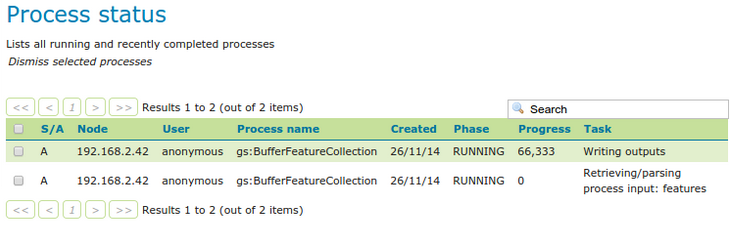
\includegraphics[width=\textwidth]{img/geoserver_status.png}
\caption{Process status page, source \cite{GS_docs}}
\label{fig:geoserver_status}
\end{figure}

\subsection{ZOO-Project}
\textit{ZOO-Project} is a WPS implementation writen in C, Python and Javascript. It is an open-source project released under MIT licence.
The platform is composed of several components:

\begin{itemize}
\item WPS Server - ZOO-kernel is a server-side implementation written in C.
\item WPS Services - ZOO-services is a set of ready-to-use web services based on libraries such as \textit{GDAL}, \textit{GRASS GIS}
or \textit{CGAL}.
\item WPS API - ZOO-API is a server-side Javascript API for creating and chaining WPS web services.
\item WPS Client - ZOO-client is a client-side Javascript library for interacting with WPS Services.
\end{itemize}

ZOO-Project is the first and in this time probably the only one full implementation of the WPS 2.0.0 standard. Apart from \textit{GetCapabilities},
\textit{DescribeProcess} and \textit{Execute} operations from WPS 1.0.0 standard it also implements \textit{GetStatus}, \textit{GetResult}
and \textit{Dismiss} operations from WPS 2.0.0.

To comply WPS 2.0.0 ZOO-Project must support synchronous/asynchronous
%% ML: To store ... - ta veta zni divne
%% AL: Prepsano.
invocation with both HTTP-GET and HTTP-POST request. There is optional 
MapServer support so an output can be stored in MapServer catalog. It is convenient to publish
results directly as WMS, WFS or WCS resources.

\subsection{ArcGIS Server}
\textit{ArcGIS Server} is server-side GIS software developed by
\textit{Esri}. It is capable of creating and managing GIS Web
%% ML: exposing ?
%% AL: opraveno
services, applications and data. It allows exposing the analytic
capability of ArcGIS to web as a \textit{Geoprocessing service}. A
%%% ML: moc mi ta veta nedava smysl
%% AL: zkusil jsem to rozdelit, je to lepsi?
geoprocessing service consists of one or more geoprocessing tasks. 
A geoprocessing task can be any ArcGIS tool. It is possible to
publish Geoprocessing service with the WPS capabilities enabled,
however only WPS 1.0.0 standard is supported.

\begin{figure}[h!]
\centering

\includegraphics[width=0.3\textwidth]{img/Intro_esri.png}
\caption{Esri logo}
\label{fig:geoserver_status}
\end{figure}

All published services have specified the minimum and maximum number of available instances. These instances run on the container machines within processes. The isolation level determines whether these instances run in separate processes or shared processes. 
\begin{itemize}
\item \textit{High isolation}- Fig. \ref{fig:arcgis_isolation_low} - each instance runs in its own process. If something causes the process to fail, it will only affect the single instance running in it.
\item \textit{Low isolation} - Fig. \ref{fig:arcgis_isolation_high} allows multiple instances of a service configuration to share a single process, thus allowing one process to handle multiple concurrent, independent requests. This is often referred to as multithreading.
\end{itemize} 

\begin{figure}[h!]
\centering
\begin{floatrow}
\ffigbox{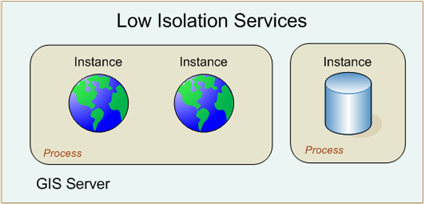
\includegraphics[width=0.5\textwidth]{img/arcgis_isolation_low.png}}{\caption{Low isolation, source \cite{AG_docs}}}{\label{fig:arcgis_isolation_low}}
\ffigbox{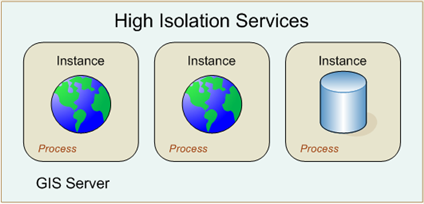
\includegraphics[width=0.5\textwidth]{img/arcgis_isolation_high.png}}{\caption{High isolation, source \cite{AG_docs}}}{\label{fig:arcgis_isolation_high}}
\end{floatrow}
\end{figure}

The advantage of low isolation is that it increases the number of concurrent instances supported by a single process. Using low isolation can use slightly less memory on your server. However, this improvement comes with some risk. If a process experiences a shutdown or crash, all instances sharing the process are destroyed. It is strongly recommended that you use high isolation.\cite{AG_docs}

\subsection{PyWPS}
PyWPS is a server-side implementation of the WPS standard written in Python. This project will be described in depth in the Sec. \ref{sec:PyWPS}.
